73. $\cfrac{(x^2-3x+8)(x^2-3x+1)}{x^2-3x}\geqslant3.$ Сделаем замену $t=x^2-3x,$ тогда $\cfrac{(t+8)(t+1)}{t}\geqslant3\Leftrightarrow$\\$
\cfrac{t^2+t+8t+8-3t}{t}\geqslant0\Leftrightarrow \cfrac{t^2+6t+8}{t}\geqslant0\Leftrightarrow \cfrac{(t+2)(t+4)}{t}\geqslant0.$ Применив метод интервалов, найдём ответ: $t\in[-4;-2]\cup(0;+\infty).$
\begin{figure}[ht!]
\center{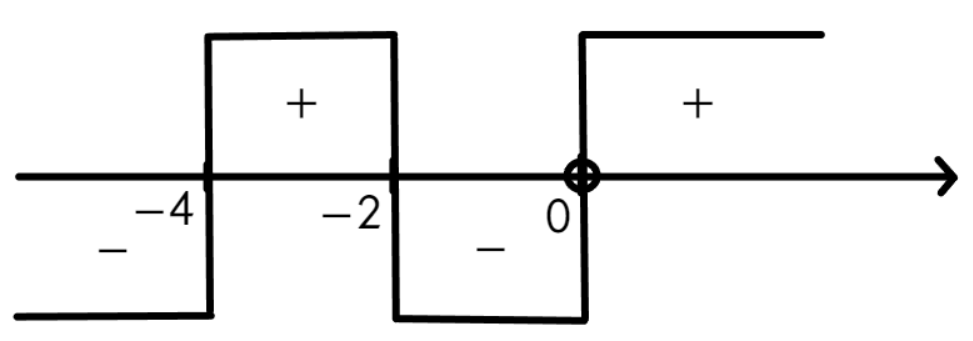
\includegraphics[scale=0.35]{ner9-73.png}}
\end{figure}\\
Теперь необходимо решить неравенства относительно $x:\ t\in[-4;-2]\Leftrightarrow\begin{cases} x^2-3x\geqslant-4,\\ x^2-3x\leqslant-2.\end{cases}
\Leftrightarrow\begin{cases} x^2-3x+4\geqslant0,\\ x^2-3x+2\leqslant0.\end{cases}\Leftrightarrow
\begin{cases} (x-1,5)^2+1,75\geqslant0,\\ (x-2)(x-1)\leqslant0.\end{cases}\Rightarrow x\in[1;2].$ Для второго интервала получим $t>0,\ x^2-3x>0,\ x(x-3)>0,\
x\in(-\infty;0)\cup(3;+\infty).$ Таким образом,  $x\in(-\infty;0)\cup[1;2]\cup(3;+\infty).$\\
